% -------------------------允许算法跨页-------------
\makeatletter
\newenvironment{breakablealgorithm}
{% \begin{breakablealgorithm}
	\begin{center}
		\refstepcounter{algorithm}% New algorithm
		\hrule height.8pt depth0pt \kern2pt% \@fs@pre for \@fs@ruled
		\renewcommand{\caption}[2][\relax]{% Make a new \caption
			{\raggedright\textbf{\ALG@name~\thealgorithm} ##2\par}%
			\ifx\relax##1\relax % #1 is \relax
			\addcontentsline{loa}{algorithm}{\protect\numberline{\thealgorithm}##2}%
			\else % #1 is not \relax
			\addcontentsline{loa}{algorithm}{\protect\numberline{\thealgorithm}##1}%
			\fi
			\kern2pt\hrule\kern2pt
		}
	}{% \end{breakablealgorithm}
		\kern2pt\hrule\relax% \@fs@post for \@fs@ruled
	\end{center}
}
\makeatother
\makeatletter
\newcommand{\rmnum}[1]{\romannumeral #1}
\newcommand{\Rmnum}[1]{\expandafter\@slowromancap\romannumeral #1@}
\makeatother

%----------------------------------------------------
\documentclass[11pt,a4paper]{ctexart}
\usepackage{fontspec}
\usepackage{xeCJK}%文字体的设置
%\newcommand{\canger}{\CJKfontspec{TsangerJinKai03}}
%\setmainfont{TsangerJinKai03} %设置全文字体
%\setsansfont{TsangerJinKai03}
%\setsansfont{TsangerJinKai03} 
%\defaultfontfeatures{Mapping=tex-text}
%\setCJKmainfont{TsangerJinKai03}
%\setCJKsansfont{TsangerJinKai03}
\usepackage{subfigure}
\usepackage{xunicode}
\usepackage{xltxtra}
\usepackage{amsmath}
\usepackage{amsfonts}
\usepackage{amssymb}
\usepackage{graphicx}
\usepackage{hyperref}
\usepackage{amsthm}
\usepackage{array}
\usepackage{tcolorbox}
\usepackage{float}   %{H}
\usepackage{booktabs}  %\toprule[1.5pt]
\usepackage[titletoc]{appendix}
\usepackage{algorithm}  
\usepackage{algorithmic}  
%\usepackage{algorithmicx}
%===================%插入代码需要的控制
\usepackage{listings}
\usepackage{xcolor}
\setmonofont{Consolas}%字体
\lstset{%
	numbers=left,
	numberstyle=\tt\tiny,%
	showstringspaces=false,
	showspaces=false,%
	tabsize=4,%
	frame=lines,%
	basicstyle=\tt\small,%
	keywordstyle=\color{ blue!70}\bfseries,%
	identifierstyle=,%
	commentstyle=\color{red!50!green!50!blue!50},%\itshape,%
	stringstyle=\color{black},%
	breaklines=true
}
%===================%

\hypersetup{
	colorlinks=true,
	linkcolor=black
}
\usepackage[left=2cm,right=2cm,top=2cm,bottom=2cm]{geometry}
\newtheorem*{solution}{解}
\newtheorem{cor}{推论}
\newtheorem{e}{习题}
\title{计算机视觉(实验三)
	
	物体分类识别和电子围栏}
\author{智科三班 \quad 严中圣 \quad 222020335220177}
\date{\today}
\begin{document}
\maketitle
\pagestyle{plain}%设置页码
%\noindent\rule{\textwidth}{1pt} %加横线
%============================================================================

%\begin{tcolorbox}[colback=white!10!white,colframe=pink!100!black]
%找任意图片,求该图片对应灰度图的边缘图。
%
%要求:
%
%1. 需要将图像转化为灰度图;
%
%2. 计算灰度图对应的边缘图;(使用3不同的算子,其中一阶和二阶算子至少各包含一个;可使用已有模块/函数)
%
%3. 观察哪种算子的效果较好,并简要说明原因。
%\end{tcolorbox}
\section{实验目的}
图像处理(image processing),用计算机对图像进行分析,以达到所需结果的技术。图像处理将会是物联网产业发展的重要支柱之一。
本实验旨在加深本课程中图像预处理、人脸检测、后处理等重要的知识点的理解和实践,并实现对视频中物体的分类识别,最终生成标注后的视频/流媒体。
\section{实验环境}
\begin{itemize}
	\item PyCharm 2022.1.3 (Professional Edition)
	\item OS: Windows 11 22H2
	\item CPU: 12th Gen Intel(R) Core(TM) i7-12700H 2.30 GHz
	\item Packages: python 3.8.15 torch>=1.7.0 torchvision>=0.8.1 numpy>=1.18.5 opencv-python>=4.1.1
\end{itemize}
\section{实验内容}
\begin{enumerate}
	\item[(1)] 对视频(固定拍摄位置)进行逐帧检测,对其中的物体进行识别;
	\item[(2)] 实现电子围栏,即对特定类别的物体进入制定区域后进行报警;
	\item[(3)] 对检测结果进行后处理,将结果在图像中进行标注,并实时播放或者保存视频;
	\item[(4)] 效率思考,若逐帧处理效率较低,考虑提高优化方法。
\end{enumerate}

\section{实验步骤}
\subsection{物体检测分类识别}
\subsubsection{目标检测算法概述}
物体检测(object detection)是计算机视觉中一个重要的分支,其大致功能是在一张图片中,用最小
矩形框框出目标物体位置,并进行分类。

物体检测的两个步骤可以概括为:
\begin{enumerate}
	\item 步骤1:检测目标位置(生成矩形框)
	\item 步骤2:对目标物体进行分类
\end{enumerate}
\begin{figure}
	\centering
	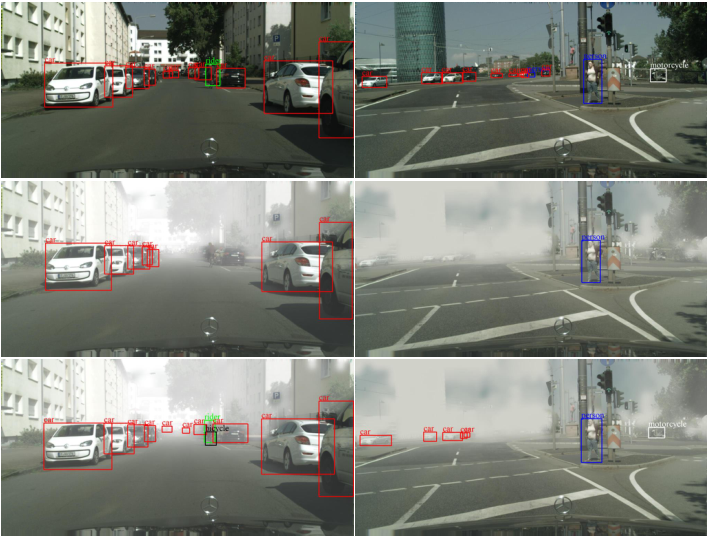
\includegraphics[width=0.7\linewidth]{screenshot010}
	\caption{目标检测任务}
	\label{fig:screenshot010}
\end{figure}

物体检测主流的算法框架大致分为one-stage 与two-stage。two-stage 算法代表有R-CNN 系列,onestage
算法代表有Yolo 系列。two-stage 算法将步骤一与步骤二分开执行,输入图像先经过候选框生成网
络(例如faster rcnn 中的RPN 网络),再经过分类网络;one-stage 算法将步骤一与步骤二同时执行,输
入图像只经过一个网络,生成的结果中同时包含位置与类别信息。two-stage 与one-stage 相比,精度高,
但是计算量更大,所以运算较慢。

为了实现物体分类识别任务,我们调用了现今最为流行的Yolov5框架进行检测,下面对Yolo算法进行介绍,完整项目见\href{https://github.com/ZS-Yan/yolov5}{https://github.com/ZS-Yan/yolov5}。
\subsubsection{Yolo 算法介绍}
\begin{enumerate}
	\item[(1)] 算法概述

	现在的大多数目标检测方式都是将物体检测问题,最后会转变成一个分类问题。在检测中,detection
	systems 采用一个classifier 去评估一张图像中,各个位置一定区域的window 或bounding box 内,是否包
	含一个物体以及包含了哪种物体。而R-CNN、Fast R-CNN 则采用的是region proposals 的方法,先生成一
	些可能包含待检测物体的potential bounding box,再通过一个classifier 去判断每个bounding box 里是否
	包含有物体,以及物体所属类别的probability 或者confidence。这种方法的pipeline 需要经过好几个独立
	的部分,所以检测速度很慢,也难以去优化,因为每个独立的部分都需要单独训练。Yolo 算法将object
	detection 的框架设计为一个regression problem。直接从图像像素到bounding box 以及probabilities。这个
	YOLO 系统如图看了一眼图像就能predict 是否存在物体,他们在哪个位置,所以也才叫You Only Look
	Once。
	\begin{figure}[H]
		\centering
		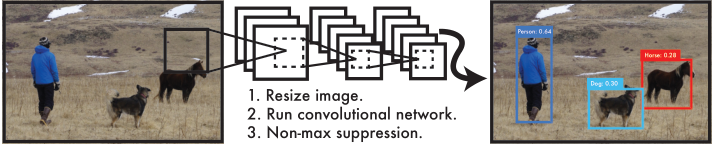
\includegraphics[width=0.8\linewidth]{screenshot009}
		\caption{Yolo 模型框架}
		\label{fig:screenshot009}
	\end{figure}
	
	这样的统一的架构,对比之前如R-CNN、Fast R-CNN 的pipeline,有以下几点好处:
	\begin{enumerate}
		\item[(1)]  YOLO 检测系统非常非常的快。受益于将detection 架构设计成一个regression problem,以及简单的
		pipeline。在Titan X 上,不需要经过批处理,标准版本的YOLO 系统可以每秒处理45 张图像;YOLO
		的极速版本可以处理150 帧图像。这就意味着YOLO 可以以小于25 毫秒延迟的处理速度,实时地
		处理视频。同时,YOLO 实时检测的mean Average Precision(mAP)是其他实时检测系统的两倍。
		
		\item[(2)] YOLO 在做predict 的时候,YOLO 使用的是全局图像。与sliding window 和region proposals 这类方
		法不同,YOLO 一次“看”一整张图像,所以它可以将物体的整体(contextual)的class information
		以及appearance information 进行encoding。目前最快最好的Fast R-CNN ,较容易误将图像中的
		background patches 看成是物体,因为它看的范围比较小。YOLO 的background errors 比Fast R-CNN
		少一半多。
		
		\item[(3)] YOLO 学到物体更泛化的特征表示。当在自然场景图像上训练YOLO,再在artwork 图像上去测试
		YOLO 时,YOLO 的表现甩DPM、R-CNN 好几条街。YOLO 模型更能适应新的domain。
	\end{enumerate}

	\item[(2)]检测方式
	
	Yolo 算法采用了Unified Detection 的方式,YOLO 检测系统,先将输入图像分成$S × S $的网格,如
	果一个物体的中心掉落在一个grid cell 内,那么这个grid cell 就负责检测这个物体。
	
	每个网格单元预测这些盒子的$B$ 个边界框和置信度分数。这些置信度分数反映了该模型对盒子是否
	包含目标的信息,以及它预测盒子的准确程度。在形式上,模型将置信度定义为$P_r(Object)×IOU^{truth}_{pred}$ 。
	如果该单元格中不存在目标,则置信度分数应为零。否则,模型希望置信度分数等于预测框与真实值之
	间联合部分的交集(IOU)。
	
	每个边界框包含5 个预测:x, y,w, h 和置信度。(x, y) 坐标表示边界框相对于网格单元边界框的中心。宽度和高度是相对于整张图像预测的。最后,置信度预测表示预测框与实际边界框之间的IOU。
	
	每个网格单元还预测$C$个条件类别概率$P_r(Class_i|Object)$。这些概率以包含目标的网格单元为条
	件。每个网格单元模型只预测的一组类别概率,而不管边界框的的数量$B$ 是多少。
	在测试时,我们乘以条件类概率和单个盒子的置信度预测,
	\begin{equation}
		P_{r}\left(Class_{i} \mid Object\right) \times P_{r}(Object) \times I O U_{pred}^{truth}=P_{r}\left(Class_{i}\right) \times I O U_{pred}^{truth}
	\end{equation}
	它为我们提供了每个框特定类别的置信度分数。这些分数编码了该类出现在框中的概率以及预测框
	拟合目标的程度。
	\begin{figure}
		\centering
		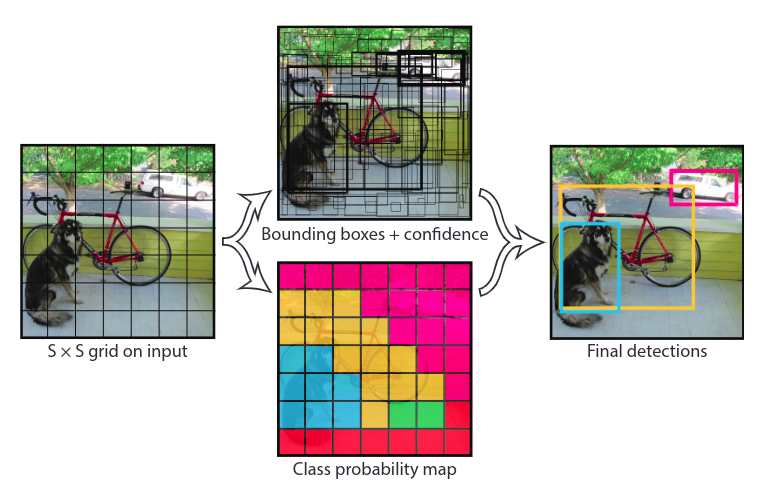
\includegraphics[width=0.6\linewidth]{screenshot011}
		\caption{Yolo 目标检测模型}
		\label{fig:screenshot011}
	\end{figure}
	
	\item[(3)] 网络结构设计
	
	Yolo 将此模型作为卷积神经网络来实现,网络的初始卷积层从图像中提取特征,而全连接层预测输
	出概率和坐标。
	网络有24 个卷积层,后面是2 个全连接层。模型只使用1×1 降维层,后面是3×3 卷积层,完整的网
	络如图所示。
	
	\begin{figure}[H]
		\centering
		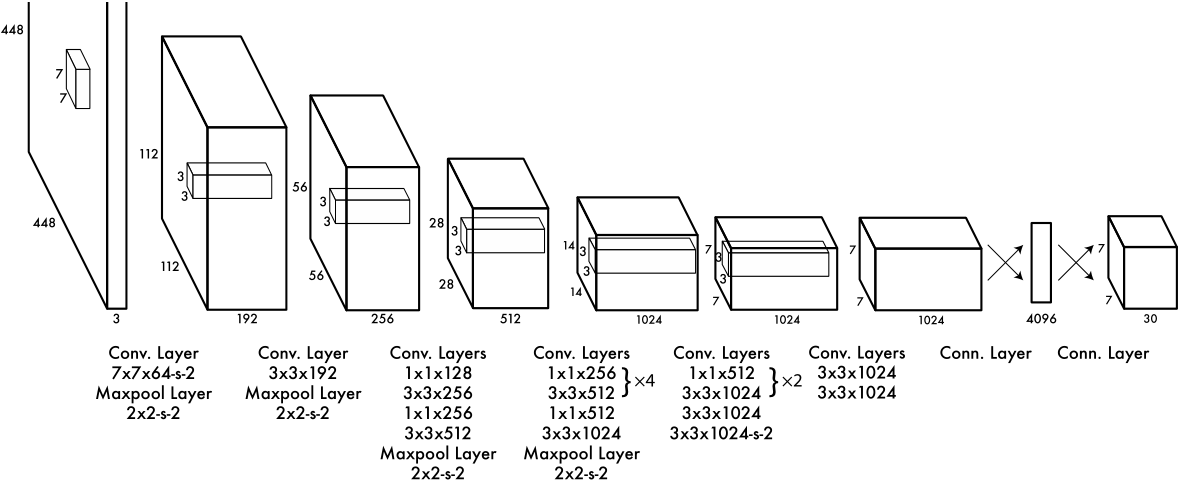
\includegraphics[width=0.7\linewidth]{screenshot012}
		\caption{Yolo 算法网络结构设计}
		\label{fig:screenshot012}
	\end{figure}
\end{enumerate}

\subsubsection{实时物体检测分类识别}
我们调用Yolov5的预训练模型对采集视频进行物体检测与分类识别,效果如下:
\begin{figure}[H]
	\centering
	\includegraphics[width=0.5\linewidth]{"test - frame at 0m13s"}
	\caption{物体检测与分类识别效果展示}
	\label{fig:test---frame-at-0m13s}
\end{figure}


\subsection{电子围栏检测报警}
为了实现电子围栏的报警检测任务,我们划定一片固定区域,实时判断该区域是否有行人经过,如检测框重叠即发出报警,实现代码如下:
\lstinputlisting[language=python]{./code/1.txt}
检测效果如下:
\begin{figure}[H]
	\centering
	\includegraphics[width=0.7\linewidth]{"test - frame at 0m6s"}
	\caption{电子围栏检测效果展示}
	\label{fig:test---frame-at-0m6s}
\end{figure}

\newpage
\begin{appendices}
\section{附录}
\subsection{物体检测代码}
%\noindent\textbf{}
\lstinputlisting[language=python]{C:/Users/11038/Desktop/yolov5/detect.py}


\end{appendices}
%\begin{lstlisting}[language=python]
%
%\end{lstlisting}


%\begin{table}[H]
%	%\caption{货舱运送设计表}\label{tab:101} \centering
%	\begin{tabular}{ccc}
%		\toprule[1.5pt]
%		     & 优点                  & 缺点                 \\
%		\midrule[1pt]
%		CCD  & 具有非常快的快门速度          & 制造工艺复杂,价格昂贵,电源消耗量高 \\
%		CMOS & 低功耗,小尺寸,总体成本低,集成度更高 & 成像过程中产生的噪声较高       \\
%		CID  & 随机访问,不会产生图像浮散       & 对光的敏感度较低        \\
%		\bottomrule[1.5pt]
%	\end{tabular}
%\end{table}
%~\\











\end{document}